
% ------------------------------------------------------------------------
% ------------------------------------------------------------------------
% abnTeX2: Modelo de Trabalho Academico (tese de doutorado, dissertacao de
% mestrado e trabalhos monograficos em geral) em conformidade com 
% ABNT NBR 14724:2011: Informacao e documentacao - Trabalhos academicos -
% Apresentacao
% ------------------------------------------------------------------------
% ------------------------------------------------------------------------


%Testando o git

\documentclass[
	% -- opções da classe memoir --
	12pt,				% tamanho da fonte
	openright,			% capítulos começam em pág ímpar (insere página vazia caso preciso)
	oneside,			% para impressão em verso e anverso. Oposto a oneside
	a4paper,			% tamanho do papel. 
	% -- opções da classe abntex2 --
	%chapter=TITLE,		% títulos de capítulos convertidos em letras maiúsculas
	%section=TITLE,		% títulos de seções convertidos em letras maiúsculas
	%subsection=TITLE,	% títulos de subseções convertidos em letras maiúsculas
	%subsubsection=TITLE,% títulos de subsubseções convertidos em letras maiúsculas
	% -- opções do pacote babel --
	english,			% idioma adicional para hifenização
	brazil				% o último idioma é o principal do documento
	]{abntex2}

% ---
% Pacotes básicos 
% ---
\usepackage{unitins}
% \usepackage{lmodern}			% Usa a fonte Latin Modern			
% \usepackage[T1]{fontenc}		% Selecao de codigos de fonte.
\usepackage[utf8]{inputenc}		% Codificacao do documento (conversão automática dos acentos)
\usepackage{lastpage}			% Usado pela Ficha catalográfica
\usepackage{indentfirst}		% Indenta o primeiro parágrafo de cada seção.
\usepackage{color}				% Controle das cores

\usepackage{graphicx}			% Inclusão de gráficos
\usepackage{subfig}
\usepackage{microtype} 			% para melhorias de justificação
\usepackage{soul}
\usepackage{amssymb}
\usepackage{amsmath}
\usepackage{spreadtab}
\usepackage{multirow}
\usepackage{amsthm}
\usepackage{url}
\usepackage{float} 
\usepackage{booktabs}

\newcommand\tab[1][1cm]{\hspace*{#1}}
% \usepackage[portuguese, ruled, linesnumbered]{algorithm2e}


% ---
		
% ---
% Pacotes adicionais, usados apenas no âmbito do Modelo Canônico do abnteX2
% ---
		% para geração de dummy text
% ---

% ---
% Pacotes de citações
% ---

%\usepackage[brazilian,hyperpageref]{backref}	 % Paginas com as citações na bibl
\usepackage[alf,abnt-etal-list=2 ]{abntex2cite}	% Citações padrão ABNT


\usepackage[table]{xcolor}
\definecolor{lightgray}{gray}{0.9}
\graphicspath{{imagens/}}

\theoremstyle{theorem}
\newtheorem{teo}{Teorema}[chapter]
\newtheorem{lema}[teo]{Lema}
\theoremstyle{definition}
\newtheorem{defi}[teo]{Definição}

% --- 
% CONFIGURAÇÕES DE PACOTES
% --- 

% ---
% Configurações do pacote backref
% Usado sem a opção hyperpageref de backref
%\renewcommand{\backrefpagesname}{Citado na(s) página(s):~}
% Texto padrão antes do número das páginas
%\renewcommand{\backref}{}
% Define os textos da citação
%\renewcommand*{\backrefalt}[4]{
%	\ifcase #1 %
	%	Nenhuma citação no texto.%
	%\or
	%	Citado na página #2.%
%	\else
	%	Citado #1 vezes nas páginas #2.%
	%\fi}%
% ---

% ---
% Informações de dados para CAPA e FOLHA DE ROSTO
% ---
\titulo{QUALIFICAÇÃO DE AMBIENTE DE ENTREGA DE APLICAÇÃO EXTERNA UTILIZANDO CONCEITO DEVOPS APLICADO AO CONTEXTO DE UMA UNIVERSIDADE PÚBLICA}
\autor{MATHEUS JOSÉ ALVES SILVA SANTOS}
\local{Palmas}
\data{2018}
\orientador{Prof. Me. Douglas Chagas da Silva}
\instituicao{%
  Universidade Estadual do Tocantins
  \par
  Curso de Sistemas de Informação
  }
\tipotrabalho{Trabalho de Conclusão de Curso (Graduação)}
% O preambulo deve conter o tipo do trabalho, o objetivo, 
% o nome da instituição e a área de concentração 
\preambulo{Projeto apresentado como requisito para aprovação na disciplina de Projeto de Conclusão de Curso de Sistemas de Informações da Universidade Estadual do Tocantins- UNITINS, sob a orientação do professor Me. Douglas Chagas da Silva.}

% ---


% ---
% Configurações de aparência do PDF final

% alterando o aspecto da cor azul
\definecolor{blue}{RGB}{41,5,195}

% informações do PDF
\makeatletter
\hypersetup{
     	%pagebackref=true,
		pdftitle={\@title}, 
		pdfauthor={\@author},
    	pdfsubject={\imprimirpreambulo},
	    pdfcreator={LaTeX with abnTeX2},
		pdfkeywords={Algoritmo}{trabalho acadêmico}, 
		colorlinks=true,       		% false: boxed links; true: colored links
    	linkcolor=blue,          	% color of internal links
    	citecolor=blue,        		% color of links to bibliography
    	filecolor=magenta,      		% color of file links
		urlcolor=blue,
		bookmarksdepth=4
}
\makeatother
% --- 

% --- 
% Espaçamentos entre linhas e parágrafos 
% --- 

% O tamanho do parágrafo é dado por:
\setlength{\parindent}{1.3cm}

% Controle do espaçamento entre um parágrafo e outro:
\setlength{\parskip}{0.2cm}  % tente também \onelineskip

% ---
% compila o indice
% ---
\makeindex

% ---

% ----
% Início do documento
% ----
\begin{document}

% Retira espaço extra obsoleto entre as frases.
\frenchspacing 

% ----------------------------------------------------------
% ELEMENTOS PRÉ-TEXTUAIS
% ----------------------------------------------------------
%\pretextual
% ----------------------------------------------------------

% ----------------------------------------------------------
% ELEMENTOS PRÉ-TEXTUAIS
% ----------------------------------------------------------
% \pretextual

% ---
% Capa
% ---
\imprimircapa
% ---

% ---
% Folha de rosto
% (o * indica que haverá a ficha bibliográfica)
% ---
\imprimirfolhaderosto
% ---

% ---
% Inserir folha de aprovação
% ---

% Isto é um exemplo de Folha de aprovação, elemento obrigatório da NBR
% 14724/2011 (seção 4.2.1.3). Você pode utilizar este modelo até a aprovação
% do trabalho. Após isso, substitua todo o conteúdo deste arquivo por uma
% imagem da página assinada pela banca com o comando abaixo:
%
% \includepdf{folhadeaprovacao_final.pdf}
%
\begin{folhadeaprovacao}

  		\includegraphics[width=1\textwidth]{imagens/unitins.png}
  		
  		\ABNTEXchapterfont\large   1. INFORMAÇÕES DO ACADÊMICO:
				
  		\normalsize Nome: Matheus José Alves Silva Santos
  		\tab Matrícula: 2015101100100005
  
  		Período VIII	
  		
  		E-mail: matheusetf@gmail.com
  		\tab Telefone: (63) 99285-7729
  		
  		\par
  		\vspace*{0.5cm}     
  		  
  		\ABNTEXchapterfont\large   2. INFORMAÇÕES DO PCC:
		  		\normalsize 
		
		Professor Orientador: Douglas Chagas da Silva
		
		Início das atividades: 13/08/2018 \tab \tab Término das atividades: 20/12/2018
		
		Total de horas semanais dedicadas ao estágio supervisionado: 20 horas
		
		Área de realização do estágio: Infraestrutura Ágil
		
		
		Data: \_\_\_\_$/$\_\_\_\_$/$\_\_\_\_
		\par
		\vspace*{0.5cm}

  		\ABNTEXchapterfont\large   3. PARECER DO PROFESSOR ORIENTADOR:
  		\normalsize 
  		
  		Aprovado $($ \tab $)$ \tab \tab Reprovado $($ \tab $)$  \tab \tab Nota: \_\_\_\_\_
  		
  	 OBSERVAÇÕES:
  		  		
  		  		 DATA: \_\_\_\_$/$\_\_\_\_$/$\_\_\_\_ \tab \assinatura{Professor Orientador}
  		\par
  		\vspace*{0.5cm}
  		 \ABNTEXchapterfont\large   4. PARECER DO COORDENADOR DE ESTÁGIO:
  		   		\normalsize 
  		
  		 OBSERVAÇÕES: 

  		 DATA: \_\_\_\_$/$\_\_\_\_$/$\_\_\_\_ \tab \assinatura{Coord. de Estágio Supervisionado}
  		 
   \begin{center}
    \vspace*{0.1cm}
    {\large\imprimirlocal}
    \par
    {\large\imprimirdata}
    \vspace*{0.5cm}
  \end{center}
  
\end{folhadeaprovacao}
% ---

% ---
% Dedicatória
% ---
\begin{dedicatoria}
   \vspace*{\fill}
   \centering
   \noindent
   \textit{ Este trabalho é dedicado à minha família, pelo apoio incondicional.} \vspace*{\fill}
\end{dedicatoria}
% ---

% ---
% Agradecimentos
% --- Es
\begin{agradecimentos}
À Deus, pela graça de permitir o meu crescimento no campo de estudo em que me sinto feliz e realizado. \\

Aos meus pais e meus irmãos que sempre apostaram em minha capacidade de crescimento e superar as barreiras que a vida impõe.\\

À minha esposa que tem sido compreensiva nos momentos de dificuldades, e companheira nos desafios que surgem.\\

Aos meus amigos e colegas de universidade, que sempre contribuíram para o desenvolvimento do meu conhecimento e pelas parcerias nos projetos e estudos.


\end{agradecimentos}
% ---

% ---
% Epígrafe
% ---
\begin{epigrafe}
    \vspace*{\fill}
	\begin{flushright}
		\textit{``Não só isso, mas também nos gloriamos \\
			nas tribulações, porque sabemos que a tribulação\\
			produz perseverança; a perseverança, um caráter \\
			aprovado; e o caráter aprovado, esperança. \\
			E a esperança não nos decepciona, porque Deus \\
			derramou seu amor em nossos corações, por meio \\
			do Espírito Santo que Ele nos concedeu.``\\
			(Bíblia Sagrada, Romanos 5:3-5)}
			
	\end{flushright}
\end{epigrafe}
% ---

% ---
% RESUMOS
% ---

% resumo em português
\setlength{\absparsep}{18pt} % ajusta o espaçamento dos parágrafos do resumo
\begin{resumo}
A demanda cada vez mais latente pela disponibilização rápida de serviços e aplicações, traz uma alta cobrança sobre a equipes de desenvolvimento e operacional quanto a quase imediata disponibilização de determinado software ao usuário final, aliado a isso a qualidade da aplicação também tem um lugar fundamental no processo. Nesse sentido, um serviço que realiza gestão da construção de uma aplicação, torna a morosidade do processo de deploy tradicional, suprida e reduz os possíveis conflitos entre as equipes de desenvolvimento e operações, a isso conferimos o termo DevOps.

Aliado a isso, o provisionamento da Infraestrutura como código e o uso de contêineres fazem com que todo o ambiente se torne replicável e escalável, assim a agilidade em todo o processo de deploy torne-se evidente e de simples monitoramento.
 

 \textbf{Palavras-chaves}: Automação, DevOps, Modelo Ágil, Integração Contínua.
 
\end{resumo}

% resumo em inglês



% ---
% inserir lista de ilustrações
% ---
\pdfbookmark[0]{\listfigurename}{lof}
\listoffigures*
% ---

% ---
% inserir lista de tabelas
% ---
% \newpage
% \pdfbookmark[0]{\listtablename}{lot}
% \newpage
% \listoftables*
% \cleardoublepage
% ---

% ---
% inserir lista de abreviaturas e siglas
% ---
\begin{siglas}
  \item DevOps - Development and Operational (Desenvolvimento e Operacional).
  \item AWS - Amazon Web Services
  \item SSH - Secure Shell
  \item NETCONF - Network Configuration
  \item CI - Continous Integracion
\end{siglas}
% ---


% ---
% inserir o sumario
% ---
\pdfbookmark[0]{\contentsname}{toc}
\tableofcontents*
\cleardoublepage
% ---



% ELEMENTOS TEXTUAIS
% ---------------------------------[!htb]-------------------------
\textual
%\rhead{\thepage}
%\pagestyle{plain}
\pagestyle{headings}
 %\pagenumbering{arabic}
%Capitulos




% ----------------------------------------------------------
% Introdução (exemplo de capítulo sem numeração, mas presente no Sumário)
% ----------------------------------------------------------


\chapter{Introdução}\label{intro}

As mudanças econômicas refletem demandas de mercado. Isso têm impacto fundamental na forma como os recursos são disponibilizados e os serviços são exigidos. Nesse sentido, a tecnologia da informação, e mais especificamente nesse estudo, a entrega de um produto ou serviço deve dar um suporte a altura das cobranças de mercado.

O cenário atual que envolve os processos de desenvolvimento e infraestrutura estão ficando cada vez mais defasados. Tradicionalmente o processo de \textit{deploy}\footnote{Publicação de um determinado software ou serviço para uso.} e gestão de entrega de soluções, tende a tornar a rotina de produção e disponibilização de serviços demasiadamente morosa. Em termos atuais, o usuário final e o próprio mercado demandam agilidade e rápida resposta.

A concepção de um modelo de entrega contínua que permita ganho na produtividade e fácil detecção de erros no processo de \textit{deploy}, tem sido cada vez mais requisitado no meio da gestão da tecnologia de informação aliado a uma cultura \textit{DevOps}\footnote{Development and Operational (Desenvolvimento e Operacional).}. Tomando isso como base, é importante entendermos que os prazos de entrega estão cada vez mais apertados, o que influi no aumento da carga de trabalho, refletindo diretamente no desempenho do profissional, tanto de desenvolvimento quanto de infraestrutura.

O presente projeto tem como foco a formulação de uma arquitetura que permita essa entrega contínua e automatizada no que diz respeito o \textit{deploy} de aplicações em tempo consideravelmente reduzido. Passa-se antes pelo estudo das diversas ferramentas disponíveis no mercado de software, a fim de levantar as possibilidades de aplicação nesse modelo.

Dessa forma é vital perceber a real vantagem no uso do modelo baseado na visão DevOps, a redução na carga de trabalho e a comunicação massiva entre os times de infraestrutura e desenvolvimento dentro de um mesmo projeto, isso resulta na entrega ágil do produto trabalhado.

A estrutura desse trabalho está organizado da seguinte forma: Na seção 2 a justificativa. Na seção 3 a problemática que envolve o tema. Na seção 4 os objetivos geral e específicos. Na seção 5 será apresentado o referencial teórico utilizado para embasar o tema e a ideia proposta, de acordo com todas as ferramentas estudadas. Na seção 6 serão apresentados os métodos utilizados para compor o estudo, assim como as ferramentas utilizadas durante todo o processo. Por fim, menciona-se as referências utilizadas no referido estudo.

\section{Objetivos}\label{cap:c_objetivos}

\subsection{Objetivo Geral }
Prover uma arquitetura integrada de ferramentas visando a disponibilização de serviços e aplicações pela Universidade Estadual do Tocantins - UNITINS.


\subsection{Objetivos Específicos}
\begin{itemize}
	\item Realizar estudos das principais ferramentas disponíveis;
	\item Definir as métricas utilizadas para avaliar o desempenho da arquitetura proposta;
	\item Detalhar as configurações e integrações de cada ferramenta que compõe a arquitetura.
	\item Compreender a prática DevOps na resolução de um problema real.
	\item Avaliar as vantagens e desvantagens da arquitetura proposta, bem como apontar a implantação da mesma em ambiente de produção.
\end{itemize}

\section{Problema}\label{cap:c_problema}

A abordagem clássica de \textit{deploy}, torna o processo lento, estressante e caro, afinal o tempo tem valor. Uma das maiores problemáticas dessa forma de disponibilização é a dificuldade em permitir uma alteração de código e imediatamente depois a sua implementação, isso porque o tempo para realizar essa atualização não permite essa agilidade, a prática adotada geralmente reúne uma série de modificações ou novas funcionalidades e o deploy a medida que essas alterações vão sendo construídas, seja semanal, quinzenal ou qualquer que seja a métrica.

Esse problema pode também ser conhecido como \textbf{"A Última Milha"}, ocorre na fase final do processo de desenvolvimento, após a validação dos requisitos e antes da implantação em produção. É exatamente nesse ponto onde são realizados os testes e homologação que o processo é notoriamente dispendioso, imagine gerir dezenas ou centenas de alterações no código onde a cobrança pela disponibilidade delas é imediata. A questão da última milha é mais notória quando adotamos uma visão macro do processo, passamos a perceber quanto tempo de se perde com etapas que podem ser automatizadas, e aliado a isso quanto recurso humano-financeiro poderia estar sendo aplicado em outra área. \cite{sato2014devops}

Em se tratando do ambiente da UNITINS, o fato que destaca a necessidade da aplicação desse trabalho, pode ser notado pelo adoção de ambientes que fazem uso de máquinas virtuais (VM). Nessa situação, há a necessidade da instalação de um Sistema Operacional (S.O) sobre uma serviço de virtualização (\textit{hypervisor}) ou disponibilização de acesso externo, via SSH ou FTP. Essa arquitetura diz respeito a cada ambiente individualmente, ou seja, cada aplicação requer que essa configuração seja feita especificamente, assim, evidencia-se o desperdício de tempo reservado para construir cada cenário. Além disso, o uso de recurso computacional é mais elevado se comparado a outras tecnologias mais recentes como \textit{contêineres}, visto que as VMs executam um S.O independente e consequentemente utilizam \textit{kernel} próprio, levando-se em consideração a execução de várias máquinas virtuais no mesmo servidor físico percebemos a necessidade de mais poder de processamento e maior uso de memória.\cite{laureano2006maquinas}


\section{Justificativa}\label{cap: justificativa}

A visão DevOps traz consigo o ideal de produtividade pela automatização na entrega de um serviço ou aplicação. Aliado a essa proposta, a Integração Contínua (CI) dá suporte para que todo o processo de construção ou \textit{build} de um código-fonte possa ser realizado de forma automatizada, desde a implantação do ambiente aos testes unitários e de integração, tal prática retira tanto da equipe de desenvolvimento quanto de infra o peso e tempo gasto no ato de disponibilizar essa aplicação para produção\cite{nathan2017}.

Fazer uso dessa abordagem possibilita aos times mencionados um retorno rápido acerca das alterações que estão continuamente sendo realizadas no código de um projeto, além de viabilizar uma forma mais barata de resolver problemas relacionados a falhas, quando identificadas.

Dessa maneira tem-se não somente a mudança do processo em si, mas, mais pontualmente uma mudança cultural. A aplicação de uma visão DevOps traz melhorias frente a compilação do código, testes automatizados, empacotamento, criação de ambientes para teste e produção, configuração da infraestrutura, migração de dados, monitoramento, auditoria, segurança, deploy, entre outros. Algumas empresas que fizeram uso das práticas DevOps passaram a ter \textit{feedbacks }significativos quanto a adaptação das mudanças do mercado, realizando diversos \textit{deploys} por dia de forma segura.\cite{sato2014devops}

Em se tratando do cenário universitário, é fundamental que a instituição corra na mesma velocidade em que as novas tecnologias surgem, em se tratando de cursos de Tecnologia da Informação isso se torna latente. Novas e boas práticas devem ser experimentadas pelos alunos, a Integração Contínua pode ser aplicada largamente para fins de estudo e experimentos, além de entenderem a vantagem do uso da automatização, podem investir um tempo maior para o desenvolvimento da aplicação.	
% ---
% Capitulo de revisão de literatura
% ---

\chapter{Referencial Teórico}\label{referencial_teorico}

\subsection{DevOps}
O conceito de DevOps, acrônimo de \textit{Development and Operations},  pode ser entendido como o nivelamento entre as equipes de desenvolvimento e operações no que tange suas interações, mantendo funções específicas, porém alinhando suas demandas referentes às responsabilidades e processos, visando a disponibilização de um produto ou funcionalidade de forma rápida e confiável.\cite{gartnerglossario}

As implementações nesse tipo de ambiente fazem uso de ferramentas de automação com o intuito de dinamizar cada vez mais a infraestrutura e torná-la mais programável, de forma que reflita na melhoria contínua da comunicação e integração entre desenvolvedores e administradores de infraestrutura, transformando o cenário tradicional de isolamento entre essas duas equipes em um ambiente participativo e colaborativo.\cite{costa}

O objetivo do DevOps é gerar em toda a equipe envolvida na produção de um software, uma cultura que vise o aumento do fluxo de trabalho (maior frequência de deploys) e em paralelo a isso, dar mais robustez no desenvolvimento da aplicação. Esse conceito representa muito mais do que simplesmente o uso de ferramentas de automação, é importante observarmos que trata-se de uma quebra de paradigmas e uma mudança na cultura no negócio com uma nova forma de produção.\cite{sato2014devops}

A agilidade no processo de deploys citado anteriormente, aluz à uma necessidade de amparo para que essa entrega rápida de fato aconteça, e mais do que isso, a demanda por parte dos clientes ou usuários de determinada aplicação, requer cada vez mais velocidade no uso de certa funcionalidade. Analogamente à revolução industrial do século XX, a mudança na forma de produção de produtos naturalmente está sendo absorvida pela tecnologia, assim, a concepção desse produto deve acompanhar a demanda externa. A adaptabilidade e mudança da arquitetura funcional no desenvolvimento de serviços tecnológicos são necessidades relevantes, a cultura DevOps é uma mudança importante nesse ponto, e a definição de um ciclo contínuo do processo, como demonstra a Figura \ref{fig:figura1}.\cite{ibmdevops}

\begin{figure}[htb] %Figura: Ciclo de vida DevOps
	\centering
	\includegraphics[width=1\linewidth]{figura1}
	\caption{Ciclo DevOps}
	Fonte: Amazon Web Services, Inc., 2018
	\label{fig:figura1}
\end{figure}

Segundo uma pesquisa realizada pelo Gartner Group sobre DevOps, em 2015, somente 29\% das organizações pesquisadas tem esse modelo atuante em produção. É evidenciado ainda que apenas 42\% desses, tem a atuação do DevOps em aplicações móveis. De acordo com o mesmo grupo o DevOps evoluiria de uma estratégia de nicho para uma estratégia comum sendo empregada por 25\% das organizações do Global 2000\footnote{Forbes Global 2000 é uma classificação anual das 2.000 empresas públicas do mundo pela revista Forbes. O ranking é baseado em quatro critérios: vendas, lucro, ativos e valor de mercado. A lista é publicada desde 2003. Fonte: Forbes}.\cite{gartnerglobal}

O uso da cultura DevOps deve ser absorvida na necessidade de versionamento contínuo de determinada aplicação, ou seja, a frequente execução de deploys. Nisso, é importante observarmos que a rápida proliferação de software requer atualizações operando na mesma medida ágil e demandada pela competitividade de mercado, visto que a velocidade no atendimento da expectativa dos clientes diferencia a empresa em relação às demais atuantes no mercado.

A principal vantagem no uso de DevOps é a melhora evidente nos processos e automatização das tarefas, otimizando o tempo e reduzindo os ciclos de desenvolvimento. Por se tratar de uma interação entre as equipes de desenvolvedores e operacionais, dizemos que é um sistema bimodal de trabalho.\cite{sato2014devops}

O monitoramento de métricas e registro de logs é um aspecto relevante. Leva-se em conta que os serviços devem estar disponíveis 24 horas por dias e durante os 7 dias da semana, acarretando em uma massiva análise de dados e logs gerados pelo sistema, portanto, a rotina na observância desses elementos deve ser constante. É possível, inclusive, a criação de alertas que apontem situações e permitam a gerência proativa dos serviços\footnote{Atividades desenvolvidas com o objetivo de produzir, executar ou disponibilizar uma ferramenta que visem atender a necessidade do usuário}.

Outro benefício fundamental do DevOps é o aumento na comunicação e colaboração que envolve todos os personagens da empresa. É importantíssimo a definição de normas que permitam um maior compartilhamento de informações, ou que permita a proliferação da comunicação, seja qual for o método ou tecnologia, desde que agregue valor. Além disso, a diminuição de ruídos na comunicação e conflitos entre as equipes melhora o ambiente e tende a produzir efeitos positivos ao fim do processo.\cite{gaea}

Pode-se ainda elencar ganhos em maior estabilidade e melhor desempenho, e tão importante quanto, a redução considerável de custos de trabalho, visto que a diminuição de tempo de produção e menor esforço afeta diretamente o custo financeiro estimado em um projeto.


\section{Infraestrutura como Código}
Falar em infraestrutura com código é exatamente absorver o entendimento do tratar a estrutura de TI como um software, programável. Com isso é possível o uso de práticas que envolvam o controle por versionamento, testes automatizados, entrega contínua, entre diversos outros recursos por meio de scripts específicos.

O uso de práticas anteriores com métodos de gerenciamento de infraestutura foram válidos e deram uma base poderosa para a concepção de novas tecnologias. Atualmente, há  uma constante demanda de softwares cada vez mais dinâmicos e um alto índice de \textit{deploys}, inclusive simultâneos, levando à necessidade de concepção de uma infraestrutura que acompanhe o ritmo de complexidade desses novos sistemas.\cite{humble2014entrega}

Segundo a Hewlett Packard\footnote{Disponível em: https://www.hpe.com/br/pt}, em seu site oficial, a infraestrutura como código elimina a necessidade de criar diversos ambientes de produção de forma manual, isolada e separadamente, e/ou atuailzações de hardware e sofware. Toda essa dinâmica pode ser feita através de scripts contidos no mesmo conjunto de códigos, trazendo velocidade, economia e otimização de tempo. Nesse contexto, a infraestrutura como código traça uma linha tênue entre o código que executa a aplicação e o código que configura um ambiente, tornando um ambiente característico do DevOps.


\section{Ferramentas para Provimento de Serviços}
Apesar do conceito DevOps ser recente, a gama de ferramentas que contribuem para implantação dessa cultura já se mostram bastante diversificadas. Dentre as mais populares, destacam-se nesta seção um conjunto de ferramentas para provimento desses serviços.

\subsection{Atlas}
É uma ferramenta disponibilizada pela Hashicorp, que tem a função de unificar projetos \textit{open source} para o manejo de aplicações finalizadas no desenvolvimento para a produção em qualquer que seja a infraestrutura.
As etapas do Atlas seguem cinco passos, como demonstra a Figura \ref{fig:etatasAtlas}, isso independe da tecnologia utilizada, sejam máquinas virtuais ou contêineres, as etapas se mantêm as mesmas. \cite{hashimoto}

\begin{figure}[htb]

	\centering
	\includegraphics[width=0.8\linewidth]{etatasAtlas}
	\caption{Etapas do Atlas}
	Fonte: Hashicorp\footnotemark
	\label{fig:etatasAtlas}


\end{figure}
	\footnotetext{Disponível em: https://www.hashicorp.com/blog/atlas-announcement}




O Atlas não é um software de caixa preta, ou seja, é possível acesso a serviços que contribuem para tanto, como Vagrant\footnote{Disponível em: https://www.vagrantup.com/} (gerencia ambientes de desenvolvimento), Packer\footnote{Disponível em: https://www.packer.io} (construção de artefatos), Terraform\footnote{Disponível em: https://www.terraform.io/} (implantação de Infraestrutura) e Consul\footnote{Disponível em: https://www.consul.io/} (monitora os serviços em tempo real).

\subsection{Chef}

É um framework destinado à automatização para sistemas e infraestrutura em nuvem. O Chef\footnote{Disponível em https://www.chef.io} constrói, entrega e administra fazendo uso de scripts replicáveis.

O Chef tira a carga dos administradores de sistemas que focam no gerenciamento projetado para servidores autônomos, ele permite executar centenas de instâncias de servidor em um tempo imensamente menor se comparado ao uso comum em deploys. Para gerenciar esse tipo de configuração, o Chef, transforma a infraestrutura em código, deixando o processo mais flexível, legível pelos analistas e testável, possibilitando assim a gerência de recursos tanto localmente quanto na nuvem.\cite{lecheta2014aws}

Em sua topologia o Chef tem três principais componentes: o Servidor Chef, as Estações e o Nós. O maior atrativo dessa ferramenta é o uso de "cookbooks" ou receitas, são ditas configurações plugáveis, que envolvem todas as instalações e parâmetros necessários para atender determinada aplicação no servidor ou máquina. Assim como as receitas convencionais definem uma estrutura sequencial que deve ser seguida a fim de tornar o produto final reflexo de uma ideia original, o Chef mantém um conceito semelhante a isso, onde define-se um estado desejado do sistema, desenvolvendo um código de configuração, então processa-se esse código, une ao processo os dados do nó em questão e garante que o estado concebido seja correspondente ao estado do sistema. \cite{garzotto2006chef}

O Chef pode ser executado em várias plataformas, como Windows, distribuições Linux, FreeBSD, Solaris, AIX, Cisco IO e Nexus. E ainda suporta plataformas em nuvem,como Amazon Web Services (AWS), Google Cloud Platform, OpenStack, IBM Bluemix, HPE Cloud, Microsoft Azure e VMware vRealize.

\subsection{Docker}

O Docker\footnote{Disponível em https://www.docker.com/} é uma plataforma de automação que implanta as aplicações em espaços isolados chamados de \textit{contêineres}, possibilitando executar as aplicações de forma mais ágil. O objetvo é criar múltiplos ambientes dentro de um mesmo servidor, acessíveis externamente.

Essa ferramenta constrói a arquitetura do software de modo a tornar o armazenamento ainda mais robusto. A essência no Docker é acomodar os serviços ou aplicações em contêineres atômicos ou descartáveis. Em todo o processo de desenvolvimento, um contêiner pode ser excluído e ser restaurado se assim surgir a necessidade, isso torna a dinâmica de entrega e testes extremamente flexível.\cite{mattiaskane}

O Docker é uma plataforma \textit{Open Source}, que não pode ser confundido com um ambiente tradicional de virtualização. No Docker fazemos uso de recurso isolados que utilizam bibliotecas do kernel em comum, isso porque é presente nessa ferramenta o Linux Containers (LXC), a Figura \ref{fig:dockerXvm} apresenta isso.

\begin{figure} [htb]
	\centering
	
	\includegraphics[width=0.8\linewidth]{imagens/dockerXvm}
	\caption{Comparativo Docker x Máquinas Virtuais}
	Fonte: Bright Computing\footnotemark
	\label{fig:dockerXvm}
	
	\footnotetext{Disponível em: http://www.brightcomputing.com/blog/containerization-vs.-virtualization-heres-our-blog-smackdown}
\end{figure}


O mesmo permite empacotar a aplicação ou um ambiente em um contêiner e movê-lo para qualquer outro host que possua o Docker instalado, tornando assim uma ferramenta portável. A grande vantagem disso é que não há necessidade de reconfigurar todo o ambiente novamente, visto que todo ele é movido, reduzindo acentuadamente o tempo de deploy de uma infraestrutura.\cite{mattiaskane}


A proposta do Docker é exatamente essa. Não há a necessidade de subir várias máquinas virtuais, tão somente precisa-se de uma máquina, e será possível executar várias aplicações sem conflitos entre elas. Todas as dependências, bibliotecas e recursos necessários especificamente a cada software, serão disponibilizados no contêiner, ver Figura \ref{fig:docker-stages}. Dessa forma, não é necessário instalar novamente todos os serviços em cada ambiente, diminui-se o uso de recursos e mantém-se as configurações da aplicação isoladas de outros softwares, evitando conflitos. \cite{scampini}

Essa plataforma não pode ser confundida com um ambiente virtualizado, visto que em cenários que utilizam máquinas virtuais há a presença de uma camada intermediária de sistema operacional entre o host e as aplicações. No Docker essa é desnecessária pois ele não utiliza kernel (vide figura 3), tornando independente quanto a nível de disco, memória e processamento.\cite{mouat}

A infraestrutura no Docker também é replicável, é possível criar imagens predefinidas e disponibilizá-las em ambientes de desenvolvimento, teste, homologação e produção para aplicações.\cite{mattiaskane}

\subsubsection{Vantagens:}
Podemos elencar alguns ganhos consideráveis na utilização do Docker :
\begin{itemize}
\item Empacotamento de software otimizando o uso das habilidades dos desenvolvedores;
\item Empacotamento de aplicação de software com todos os arquivos e dependências necessárias para determinada aplicação.
\item Utilização de artefatos empacotados que possibilitem a passagem pelo teste e produção sem necessidade de recompilação.
\item Uso de softwares sem onerar recursos demasiados, visto que o contêiner é apenas um processo que se comunica diretamente com kernel do Linux.
\end{itemize}

\begin{figure}[htb]
	\centering
	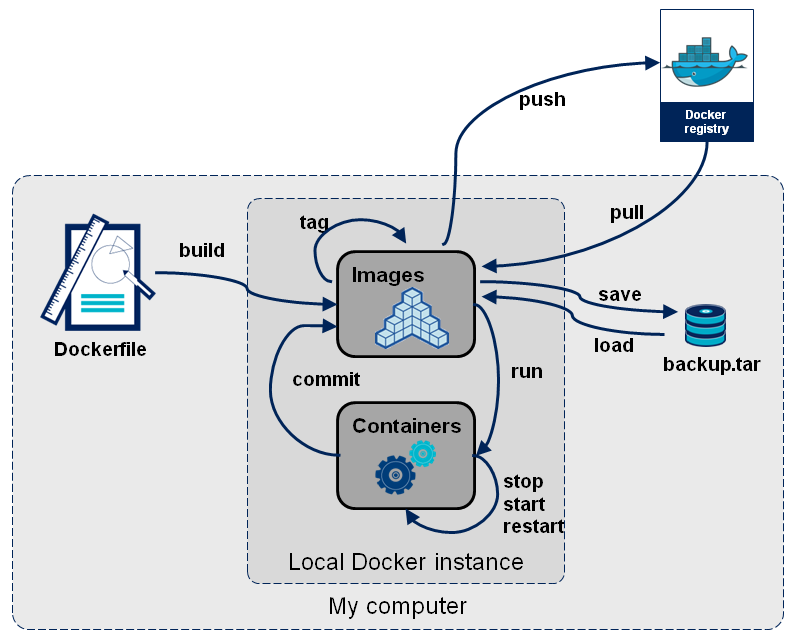
\includegraphics[width=0.7\linewidth]{imagens/docker-stages}
	\caption{Fluxo de disponibilização de Imagem Docker}
	Fonte: OCTO Technology\footnotemark	
	\label{fig:docker-stages}
	
	\footnotetext{Disponível em: https://blog.octo.com/en/docker-registry-first-steps/}
\end{figure}
\newpage
\subsection{Puppet}
É uma ferramenta de código livre para gestão de configurações. A ideia central do Puppet\footnote{Disponível em https://www.puppet.com/} é a administração de diversas máquinas físicas ou virtuais, onde a configuração é centralizada em um único nó e então distribuídas por diversos nós na rede, assim, gerenciando configurações, automatizando instalação de pacotes e facilitando o estabelecimento de normas e auditoria.\cite{walberg2008automate}

A ferramenta está disponível em duas versões: Puppet Enterprise\footnote{Disponível em: https://puppet.com/products/puppet-enterprise} (com suporte pago), e a Open Source Puppet\footnote{Disponível em: https://puppet.com/download-open-source-puppet} (código aberto). É uma ferramenta bem utilizada pela comunidade e por isso existem muitos módulos desenvolvidos, empresas como McAfee e Nasa fazem uso dela.

O Puppet utiliza o serviço SSH para a conexão aos hosts, esse é um ponto positivo se olharmos pela ótica que em alguns cenários não é possível a instalação de agentes ou em situações onde o agente consome uma fatia considerável de memória e cpu.\cite{puppet}

\begin{table}[h]
	\centering

	\begin{tabular}{|p{3.0cm}|p{3.0cm}|p{3.0cm}|p{3.0cm}|}
		\cline{1-4}
		
		  & Ansible &Puppet & Chef \\ % Note a separação de col. e a quebra de linhas
		\hline                               % para uma linha horizontal
		Linguagem do Script & YAML        & Custom DSL baseado em Ruby & Ruby\\ \cline{1-4}
		
		Infraestrutura & Máquina controladora aplica configuração em nós via SSH  & Puppet Master sincroniza configuração em nós Puppet & Chef Workstation empurra configuração para o servidor Chef onde os nós Chef serão atualizados  \\ \cline{1-4}
		
		Softwares especializados requeridos para nós & Não & Sim & Sim\\ \cline{1-4}
		
		Fornece ponto de controle centralizado & Não, qualquer computador pode ser controlado &  Sim, via  Puppet Master & Sim, via servidor Chef \\ \cline{1-4}
		
		Terminologia de Scripts & Playbook/Roles & Manifests/ Módulos & Receitas/ Cookbooks \\ \cline{1-4}
		
		Ordem de Execução das Tarefas & Sequencial & Não sequencial & Sequencial \\ \cline{1-4}         
		
	\end{tabular}
	\caption{Comparativo entre Ferramentas de Gerenciamento de Configurações}
	Fonte: Digital Ocean\footnotemark
\end{table}
	\footnotetext{Disponível em: https://www.digitalocean.com/}


\subsection{Ansible}

O Ansible\footnote{Disponível em https://www.ansible.com} foi criado em 2012, por Michael DeHann, basicamente essa ferramenta gerencia configurações e orquestra tarefas. Nesse sentido ele implementa módulos para nós sobre SSH. Os módulos são distribuídos nos nós temporariamente que realizam a comunicação com a máquina de controle (assim com em ferramentas concorrentes) por meio de um protocolo JSON\footnote{Disponível em: http://jsonapi.org/}.\cite{imhofsurvey}

O diferencial do Ansible em relação as demais ferramentas que se propõe ao mesmo objetivo, é que ele atua com uma arquitetura cliente-servidor, sem agente,  isso que dizer que os nós não são necessários para a instalação dos daemons para comunicação com a máquina controle. Isso resulta em diminuição de carga na rede. 

Os objetivos mais notáveis do Ansible é tornar a experiência do usuário muito mais simples e fácil, e investir massivamente na segurança e confiabilidade utilizando o \textit{OpenSSH} como condutor de dados. É uma linguagem construída tendo como parâmetro a auditabilidade, ou seja, possibilitar ao analista o acompanhamento de todas as etapas, rotinas e dados circulados dentro de uma arquitetura definida.\cite{marcelocosta}

Nessa ferramenta ainda encontramos o uso de um arquivo de inventário, denominado "hosts", que definem quais nós serão gerenciados, que é simplesmente um arquivo de texto que lista os nós individualmente ou agrupados, ou até um arquivo executável que constrói um inventário de hosts. É uma opção de alta confiabilidade e segurança, e isso se fundamenta pelo uso do \textit{Secure Shell}. Possui ainda fácil usabilidade, no entanto, não deixa a desejar em qualquer aspecto se comparado a soluções concorrentes.

Na forma tradicional de trabalho o Ansible faz o \textit{upload} do código que deve ser executado nas estações clientes, é então executado, retorna o resultado da execução e após isso é removido dos clientes. Quando usamos a ótica DevOps esse tipo de fluxo é modificado, fazendo uso do protocolo NETCONF\footnote{Disponível em: https://tools.ietf.org/html/rfc6241} (RFC 6241), onde é possível o envio de comandos aos componentes e receber o retorno da aplicação.

\subsubsection{Componentes}
O Ansible é estruturado pela composição dos seguintes elementos:

\begin{itemize}
	\item Playbooks\footnote{Disponível em https://docs.ansible.com/ansible/playbooks.html}: arquivos de configuração, implementação e linguagem de orquestração do Ansible.
	\item Agentless\footnote{Disponível em https://dbruno.ansible.com/ansible/}: É descartado o uso de agente nos servidores a serem monitorados. Isso deve-se à utilização de \textit{OpenSSH} para definir o estado atual do ambiente, adaptando-se se acaso estiver em desconformidade com a configuração no playbook.
	\item Módulos\footnote{Disponível em https://docs.ansible.com/ansible/modules.html}: São as tarefas executadas de fato. Os módulos são ditos como "plugins de tarefas" e por isso são eles que realizam as atividades pertinentes.
	\item Inventário\footnote{Disponível em https://dbruno.ansible.com/ansible/}: Armazena e controla informações sobre os grupos de hosts.
\end{itemize}

\subsubsection{Vantagens}
Podemos apontar alguns ganhos consideráveis na utilização do Ansible.
\begin{itemize}
	\item Não há a necessidade na instalação de agentes nos servidores a serem gerenciados;
	\item Gerencia paralela e simultaneamente de forma orquestrada; 
	\item Simples configuração e bem estruturado;
	\item Desenvolvimento em diversas linguagens.
\end{itemize}

\subsection{GitHub }
É um dos serviços web de repositórios mais difundidos. Com essa ferramenta é possível hospedar projetos e aplicações, trabalhando com controle de versionamento.

O Github\footnote{Disponível em https://www.github.com} funciona por meio de repositórios, que se dividem em pastas e dentro destas, subpastas que comportam os arquivos de diversas extensões e linguagens. Ainda oferece a possibilidade de contribuir com um código mesmo que não seja membro original do projeto, desde que permitido. Além de permitir o acesso múltiplo por diversos desenvolvedores de uma mesma empresa, permitindo que vários programadores trabalhem simultaneamente em uma mesma aplicação ou arquivo.\cite{bell2015introduccao}

Essa ferramenta funciona através de comandos "git", que gera ações de \textit{upload, request, clone, update, remove, merge e rollbacks} (retorno a versões anteriores do código). O git é estruturado em árvores, e nessa estrutura encontramos os \textit{Branchs} que são ponteiros que apontam para um determinado commit, como demonstra a Figura \ref{fig:git}

\begin{figure} [htb]
	\centering
	\includegraphics[width=0.85\linewidth]{git}
	\caption{Fluxo commit e request}
	Fonte: Cloud Turbine\footnotemark
	\label{fig:git}
\end{figure}
	\footnotetext{Disponível em: https://www.cloudturbine.com/using-github-and-git/}

\subsection{Jenkins}

Essa ferramenta multiplataforma funciona como um servidor destinado a integração contínua que automatiza a execução de tarefas, possui código aberto e permite ao usuário total liberdade em sua operação.

Basicamente o Jenkins\footnote{Disponível em https://www.jenkins.io} atua em um conceito de integração contínua, onde o objetivo é agilizar tarefas que tradicionalmente demandam um tempo de excecução mais prolongado como compilação do projeto e execução de testes automatizados. Cada interação é analisada por um \textit{build} automatizado a fim de detectar possíveis erros de integração, isso permite que testes sejam realizados reduzindo problemas de updates e tornando o software mais coeso.\cite{atalay}

O Jenkins pode ser integrado ao Git, SVN, CVS, Maven, entre outros. É importante ressaltar que um ponto forte do Jenkins é a difusão entre a comunidade. Ele ainda possui mais de 1000 plugins disponíveis e utilizado por várias empresas de desenvolvimento de softwares.\cite{ouverney2018automaccao}

Um recurso interessante é o uso de \textit{Forks} (recurso do GitHub), que permitem a criação de cópias de um determinado projeto e trabalha nesse sem a preocupação de afetar em algum ponto a aplicação original. É possivel ainda, adicionar testes de desempenho e balanceamento na integração contínua, permitindo a análise de risco e a reduzir eventuais quedas de performance no momento em que um novo recurso é adicionado ou a correção de um erro presente.\cite{ouverney2018automaccao}

\subsubsection{Vantagens}
As principais vantagens do Jenkins podem ser destacadas abaixo:
\begin{itemize}
\item \textit{Builds} periódicos;
\item Testes automatizados;
\item Possibilita análise de código;
\item Identificar erros mais cedo;
\item Fácil de operar e configurar;
\item Comunidade ativa;
\item Integra outras ferramentas por meio de plugins nativos.
\end{itemize}

\subsection{Sonar}

O SonarQube\footnote{Disponível em: https://www.sonarqube.org/} é uma plataforma de análise da qualidade do código, com ele é possível avaliar por meio de dados estatísticos o desempenho de determinada aplicação quanto aos testes realizados utilizando diversas métricas. 

A qualidade do código é verificada através de alguns eixos, como na Figura \ref{fig:7axessonar}, sendo esses, a arquitetura, duplicações de código, complexidade, regras de codificação, comentários, testes unitários e erros em potencial.

\begin{figure}[htb]
	\centering
	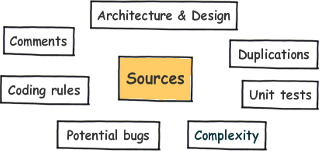
\includegraphics[width=0.5\linewidth]{imagens/7axes_sonar}
	\caption{7 Eixos de Análise do Sonar}
	Fonte: Blog Gabriel Amorim\footnotemark
	\label{fig:7axessonar}
\end{figure}
	\footnotetext{Disponível em: http://blog.gabrielamorim.com/analisando-a-qualidade-do-codigo-com-o-sonar/}

O Sonar tem compatibilidade com diversas linguagens, e plugins para vários serviços como Jenkins, por exemplo. Assim, é possível através da execução de uma determinada tarefa, definir métricas de análise, monitorar todo o processo e como retorno disponibilizar dados estatísticos referente a cada teste executado.\cite{cabralrelato}

Vantagens:
\begin{itemize}
	\item Fácil acompanhamento da evolução do código;
	\item Representação dos dados através de gráficos;
	\item Uso simples da ferramenta.
\end{itemize}

\subsection{Kubernetes}

O Kubernetes\footnote{Disponível em: https://kubernetes.io/} é um sistema destinado à orquestração de contêineres. É perfeitamente associável a ferramentas como Docker, Rocket, Jenkins, Chef, Puppet e Ansible. O seu objetivo é retirar o peso de execução de determinado contêiner em uma única instância do serviço, para isso o Kubernetes cria nós ou slaves diferentes e distribui a execução da tarefa entre esses nós. A figura \ref{fig:kubernetes} demonstra a arquitetura comum do Kubernetes.

\begin{figure}[htb]
	\centering
	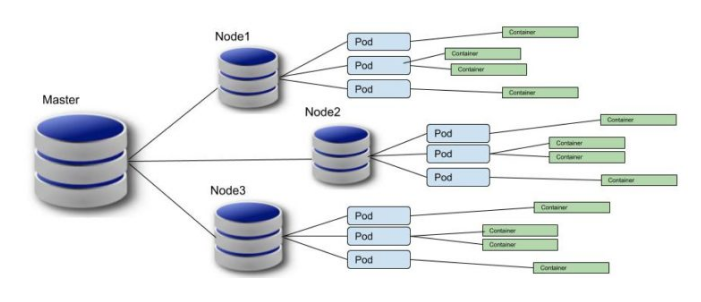
\includegraphics[width=1\linewidth]{imagens/kubernetes}
	\caption{Arquitetura do Kubernetes}
	Fonte: King Host\footnotemark
	\label{fig:kubernetes}
\end{figure}
	\footnotetext{Disponível em: https://king.host/blog/2018/05/introducao-ao-kubernetes/}

Instituições como \textit{Google} revelaram que utilizam  contêineres em serviços como \textit{Gmail} e \textit{Google Docs}, nesses são mais de 2 bilhões de implantações por semana, essa dinâmica é gerida pelo Borg, e essa mesma ferramenta foi precursora do Kubernetes. Em 2015 foi doada para a \textit{"Native Computing Foundation"} e \textit{"Linux Foundation"}, sendo a partir disso um projeto\textit{ open source}.\cite{trucco}
\newpage
Conforme a Figura \ref{fig:kubernetes}, a arquitetura do Kubernetes pode ser definida como:
\begin{itemize}
\item \textbf{Master:} é a instância central que provê uma determinada aplicação com configurações específicas.
\item \textbf{Cluster: }conjunto dos componentes. Na figura \ref{fig:kubernetes} percebemos a criação de um cluster.
\item \textbf{Node:} Uma máquina ativa gerenciada pelo master, pode também ser mencionada como \textit{minions} ou \textit{slaves}.
\item \textbf{Pods:} menores unidades implantadas que podem ser criadas, escaladas e manuseadas. É uma coleção lógica de contêineres que pertencem a uma aplicação.
\end{itemize}

O principal motivo que atrai desenvolvedores para o uso do Kubernetes é viabilizar aos \textit{clusters} abranger alocações em clouds públicas, privadas ou híbridas, e mais especificamente ainda, quando essa arquitetura envolve uma gama elevada de contêineres, o que exige que a ferramenta seja obrigatoriamente auto-escalável e proporcione alta disponibilidade.\cite{netto2016replicaccao}

\subsubsection{MiniKube}
O manuseio do Kubernetes é mais complexo do que seu concorrente direto \textit{Docker Swarm}\footnote{Disponível em: https://docs.docker.com/engine/swarm/}, demanda mais conhecimento de redes e sistemas distribuídos do arquiteto projetista do ambiente.

Pensando nisso a comunidade criou o Minikube\footnote{Disponível em: https://kubernetes.io/docs/setup/minikube/}, que basicamente é uma \textit{Toolkit} que reúne uma série de soluções que facilitam muito a implantação do Kubernetes, isso tornou a aplicabilidade mais abrangente, sendo possível o uso em plataformas Windows, Linux e Mac. Nesse caso, o Minikube simula um nó com tudo o que é preciso já instalado e configurado.\cite{mceniry2017kubernetes}


Vantagens:
\begin{itemize}
\item Fácil manipulação de contêineres;
\item Escalonamento da aplicação;
\item Volumes persistentes;
\item Auto regeneração;
\item Abstração de complexidade.
\end{itemize}

Desvantagens:
\begin{itemize}
\item Pouca documentação disponível para iniciantes;
\item Curva de aprendizado longa;

\end{itemize}




% ---
% Capitulo de METODOLOGIA
% ---




\chapter{Metodologia}\label{cap:metodologia}

No âmbito desse estudo, é proposta uma arquitetura para implantação de hospedagem de aplicações externas. Assim, o levantamento de informações consistiu em avaliar um conjunto de requisitos essenciais para apoiar o modelo apresentado.

Para a eleição das ferramentas escolhidas foi levado em conta, a sua disponibilização de código open source, a flexibilidade no uso e confiabilidade nos resultados, as suas vantagens e desvantagens, a aceitação junto a comunidade científica e a documentação disponível, seja por meio de livros ou artigos publicados ou por contribuições junto a comunidade web.

O processo de escolha das ferramentas teve como ponto inicial estar em consonância com atuabilidade do mercado de TI e ter continua contribuição da comunidade web. Sendo assim, o primeiro critério a ser considerado foi como a ferramenta daria suporte às diversas linguagens de programações disponíveis. Outro fator relevante está atrelado a maneira como o produto pode ser adquirido, mais diretamente, ao custo necessário para fazer uso da ferramenta. A premissa é que as mesmas deveriam possuir versão open source que  dessem suporte às necessidades da arquitetura proposta.

Dessa forma, alguns requisitos foram considerados na escolha, os pontos citados a seguir nortearam a escolha: 
    \vspace*{0.5cm}

\begin{itemize}
	
	\item Extensibilidade: tomando como fato as rápidas mudanças no cenário tecnológico, a ferramenta deveria poder dar suporte a diferentes linguagens e integrações;
	\item Usabilidade: a ferramenta deveria ser de fácil compreensão e fornecer uma boa experiência ao usuário;
	\item Segurança: é essencial que critérios de segurança sejam inerentes à ferramenta, definição de papéis e usuários.
	
\end{itemize}

    \vspace*{0.5cm}

\section{Materiais Utilizados}

Tomando por base os critérios mencionados no item 6, passou-se a definição das ferramentas, sendo essas:



\begin{table}[htb]
	    \vspace*{0.5cm}
	
	\centering
	\begin{tabular}{l|c}
		\hline
		\multicolumn{1}{c}{DESCRIÇÃO} & ESPECIFICAÇÃO                                                                                            \\ \hline
		Máquina Física                  & \begin{tabular}[c]{@{}c@{}}Mac OS High Sierra 10.13.4 /\\ i5 2.4Ghz 10 GB RAM 1333 MHz DDR3\end{tabular} \\ \hline
		Oracle VirtualBox               & Versão 5.2.8                                                                                             \\ \hline
		Docker                          & Versão  17.12.0-ce                                                                                                 \\ \hline
		GitHub                          & Serviço Web: www.github.com                                                                              \\ \hline
		SonarQube                          & Plugin Jenkins Versão 2.8.1                                           \\ \hline
		Jenkins                          & Versão 2.11.2                                        \\ \hline
		Kubernetes                          & Plugin Jenkins - Minikube Versão 1.11                                           \\ \hline
	\end{tabular}
\caption{Ferramentas utilizadas}
\end{table}

\begin{itemize}
	    \vspace*{0.5cm}
	
\item VirutalBox: Criação de máquinas virtuais para testes. Serão construídas máquinas virtuais para execução dos hosts clientes e servidores;
\item GitHub: Versionamento e repositório. Esse serviço receberá os códigos das aplicações dos desenvolvedores;
\item Jenkins: Automatização da execução de tarefas e testes de implantação. O Jenkins será executado em uma máquina virtual com Sistema Operacional Ubuntu Linux 64 bits.
\item Docker: Contêineres para armazenamento das aplicações e serviços. O Docker será executado em uma máquina virtual com Sistema Operacional Ubuntu Linux 64 bits.
\item Kubernetes: Recurso utilizado para criar nós ou slaves, destinados a dividir o peso de compilação, evitando a sobrecarga no nó master do Jenkins, utilizar-se-á versão Minikube.
\item Sonar: Plugin de análise estatística do build, com ele será possível coletar resultado das métricas definidas para resultados.

\end{itemize}

    \vspace*{0.5cm}

\section{Arquitetura }

Para o ritmo do processo de deploy será considerada a arquitetura representada na figura 8, que envolve desde a requisição do ambiente por meio de formulário até o provisionamento e entrega.
Toda a arquitetura é gerida e orquestrada pelo Ansible desde uma nova mudança no repositório do GitHub até o envio para produção.
\\
\begin{figure}
	\centering
	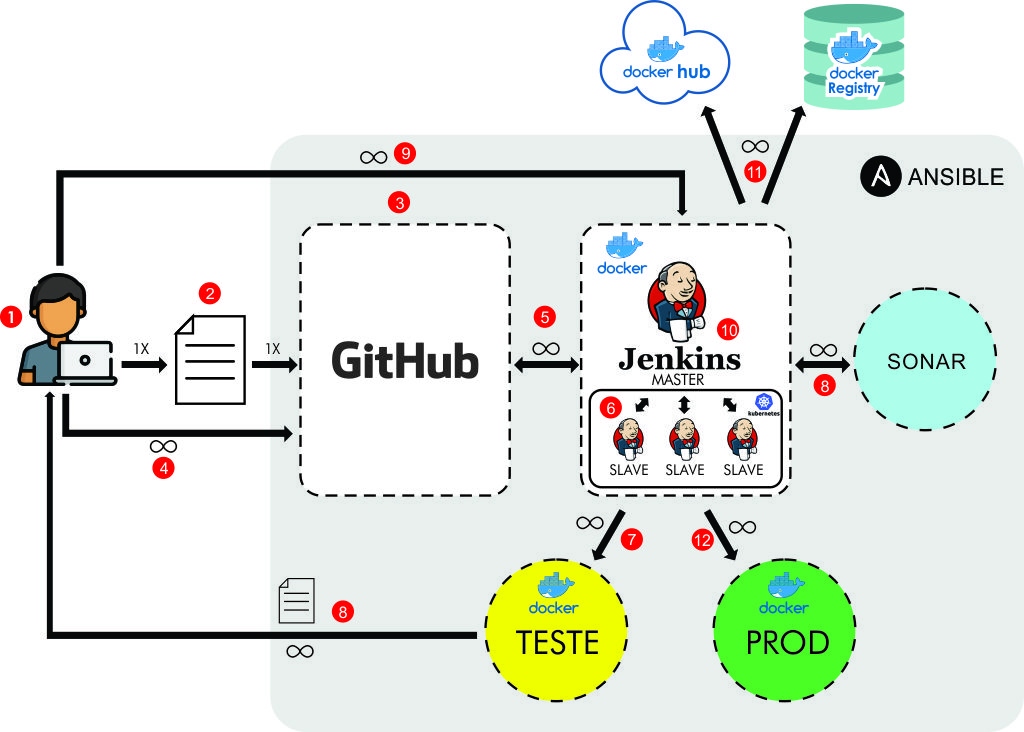
\includegraphics[width=1\linewidth]{imagens/pipelinejenkins}
	\caption{Representação da Arquitetura Proposta}
Fonte: Acervo próprio
	\label{fig:pipelinejenkins}
\end{figure}

Considerando o modelo apresentado na figura 8, pontuaremos cada etapa a fim de detalhar o fluxo da disponibilização ao usuário final. O simbolo de infinito encontrado no na mesma figura, indica que o fluxo nesse ponto é contínuo e se repete a cada nova interação.

\begin{enumerate}
	\item No ponto de partida, é pre-requisito a existência de conteúdo codificado em linguagem de programação, que permita o versionamento do projeto.
	\item O desenvolvedor faz a requisição de um novo ambiente através de formulário web, que contenha as informações pertinentes, tais como link do repositório, dependências do projeto e informações de acesso à aplicação.
	\item A requisição é recebida pelo provedor que verifica os dados de solicitação, avalia a disponibilidade de repositório;
	\item O desenvolvedor envia os commits e o GitHub gera uma notificação de alteração ao Jenkins;
	\item Jenkins recebe a notificação (Git Fetch – Git Merge – Dry Run – Commit Check);
	\item O Jenkins cria instâncias diferentes para construir o projeto, para isso, faz uso do Kubernetes;
	\item O Jenkins incia o build e realiza testes automatizados;
	\item O gestor é notificado quanto aos logs e status do build;
	\item O gestor homologa ou não o build;
	\item Jenkins gera novo release e nova tag de versão;
\item O Ansible informa ao Docker para construir uma nova imagem da aplicação e a envia para um repositório no Docker Hub\footnote{Disponível em: https://hub.docker.com/}
	\item Estando as alterações aprovadas o Jenkins através do Ansible realiza deploy da aplicação em um contêiner Docker destinado a produção;
\end{enumerate}

O processo inicia com a chamada de uma nova requisição do código-fonte do aplicativo do repositório Github em questão. Após isso faz-se a atualização da versão do projeto levando-se em conta o número de compilação, assim tem-se uma identificação digital específica para essa implantação. Após a atualização da versão do projeto, o Jenkins inicia a construção do código fonte.
    \vspace*{0.5cm}

\section{Descrição do Serviço de Integração Contínua}

A fim de criar uma plataforma que possibilitasse a construção e configuração de um ambiente replicável, auto escalável e ágil, foi utilizado o conceito da infraestrutura como código, ou \textit{"as-a-code"}. Nesse sentido, vislumbrou-se um serviço que reunisse as ferramentas Docker, Jenkins e Kubernetes sob orquestração do Ansible para realizar a execução do processo de deploy bem como o provisionamento do ambiente com a instalação dos serviços, dependências e configurações com a chamada do arquivo Dockerfile que faz a instalação das dependências para o ambiente Jenkins, bem como as chaves de acesso, instalação de plugins, busca por jobs, e criação dos devidos contêineres Docker. 

O ponto de partida é a criação do \textit{Formulário de Solicitação de Ambiente de Desenvolvimento}, no qual o usuário sinalizará a pretensão de alocação de sua aplicação em servidor web local. Os dados informados nesse formulário gerarão um arquivo \textit{.json} que será lido pela API do Jenkins a fim de se criar um novo Job para esse repositório, esse ponto será mais detalhado na subseção 3.3.1.

Os arquivos fundamentais desse projeto são primeiramente o playbook (cd.yml) do Ansible, ele é responsável por fazer a instalação do Docker e baixar a imagem Jenkins, e então iniciar o processo de configuração do ambiente chamando o Dockerfile mencionado anteriormente. É necessário criar uma conta no Docker Hub\footnote{hub.docker.com}, esse será o repositório onde as imagens Docker serão exportadas e servirá como controle de versionamento da imagens\footnote{Nesse caso o repositório fará versionamento da imagem do serviço, não do código-fonte, esse será feito diretamente no GitHub}.

A imagem do Jenkins foi construída com o objetivo da mesma ser replicável e auto-escalável, isso quer dizer que a mesma possui configurações genéricas e, portanto, aplicável em qualquer tarefa a ser executada, sendo os \textit{Playbooks }Ansible de cada serviço responsável por suprir as dependências de cada projeto não disponíveis no Jenkins.

O arquivo Dockerfile traz o script utilizado para construir as imagens Docker e mapear os volumes externos utilizados pelo Jenkins, como arquivos de configuração e base de dados, além disso esse arquivo inicia os contêineres dos serviços com o comando "run". O arquivo \textit{plugins.txt}\footnote{vide Apêndice A} mapeado para um desses volumes traz uma lista de plugins que serão instalados em tempo de execução no build da imagem, assim o Ansible somente instalará plugins mencionados no formulário e que não conste nessa lista, nesse caso é realizado um novo build da imagem para atualizar a lista de plugins e/ou demais configurações.

Na raiz do projeto estão os arquivos de configuração do Jenkins. Nesses, estarão os parâmetros necessários para iniciar o serviço do Jenkins sem a necessidade de reconfigurar toda a ferramenta ao reinicio de cada instância. Essa forma de configuração torna o serviço reaproveitável, ou seja, tanto é possível criar um padrão inicial definido para demais projetos do Jenkins, quanto utilizá-lo para execução dos mais diversos tipos de jobs, desde o mais básico ao mais complexo, alocando somente o recurso necessário para cada iteração, dessa forma não se desperdiça recurso computacional para os builds mais simples e utilizam-se instâncias diferentes do Jenkins através de \textit{slaves} orquestrados pelo Kubernetes para construções que demandam mais poder computacional.
    \vspace*{0.5cm}

\subsection{Pipeline do Build}

Para início do processo de build do código, é necessário antes de tudo que esteja disponível um repositório de versionamento de códigos, definido aqui com a plataforma do GitHub. Essa sinalização será concebida por meio de um \textit{Formulário de Solicitação de Ambiente de Desenvolvimento}. Esse formulário será disponibilizado por um endereço web, onde é premissa que o usuário já possua um repositório para o projeto no GitHub, e preencha os demais campos solicitados do formulário. É requerido desde o nome do responsável pelo projeto até as dependências necessária para execução do mesmo. Essa busca pelos Jobs são feitas pela API do Jenkins semelhantemente ao REST.

Nesse sentido a API pode ser usada para:

\begin{itemize}
	\item Recuperar informações de Jenkins para consumo programático;
	\item Desencadear uma nova compilação;
	\item Criar ou copiar Jobs.
\end{itemize}


\begin{figure}[htb]
	\centering
	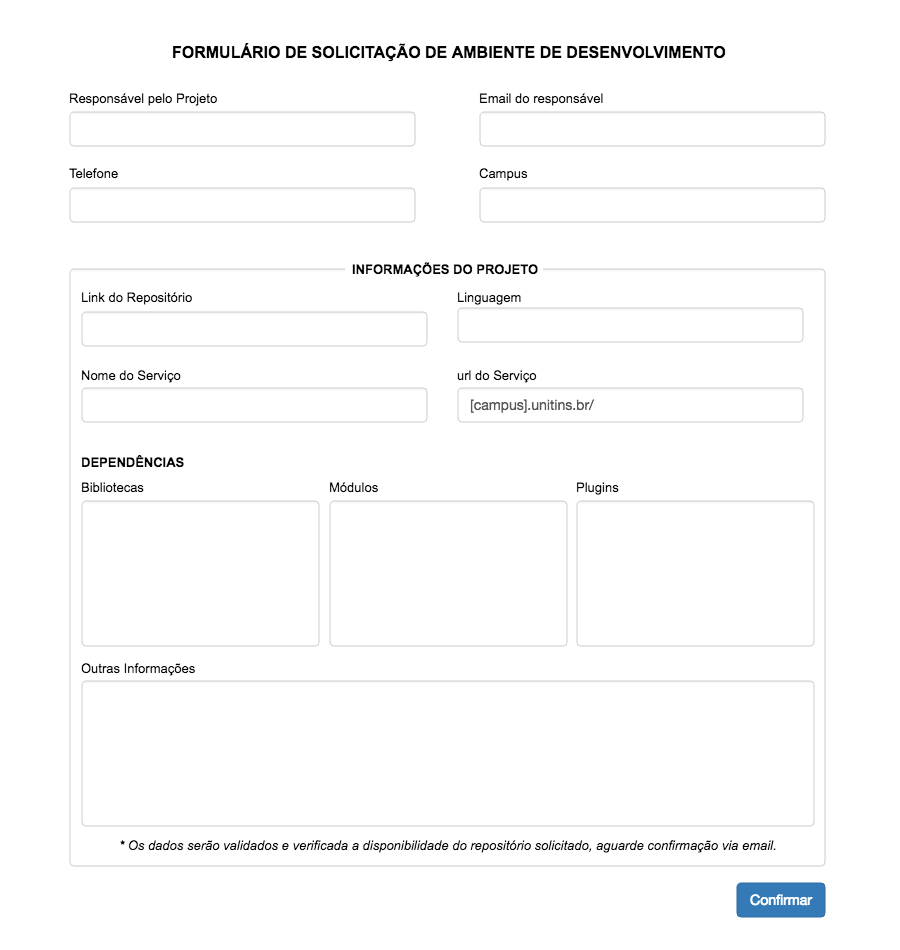
\includegraphics[width=1\linewidth]{imagens/formulario}
	\caption{Formulário Web para Solicitação de Provisionamento de Ambiente}
	\label{fig:formulario}
	
\end{figure}


O Pipeline de um projeto baseia-se num fluxo iniciado na alteração do estado do código-fonte em um repositório até a disponibilização do software em produção. Esse processo tem por natureza um fluxo contínuo da cadeia de comandos da Integração Contínua. Iniciando, o Jenkins é responsável por monitorar o repositório GitHub a fim de verificar alteração no estado do código do projeto utilizando recurso de \textit{Push Notification} já próprio da ferramenta, ou seja, se houveram \textit{commits} no mesmo, o Jenkins atualiza a versão do projeto de acordo com o número de compilação, dessa forma garantisse uma assinatura única da construção durante o processo de implantação. Após atualizar a versão do código partiremos para a construção do mesmo.

Tendo sucesso na compilação, partiremos para a construção do projeto. Após o Jenkins identificar uma alteração no código, o mesmo clona o projeto do repositório, e escalona diferentes estâncias desse mesmo serviço, fazendo o papel de \textit{slaves} e o \textit{master} faz o papel de orquestrador, esse processo retira o peso e custo computacional, se o projeto fosse compilado somente em uma instância master do Jenkins, assim o build é distribuído entre os \textit{slaves} e ao final do processo realiza o \textit{merge} do projeto, esse processo é gerenciado pelo \textit{Kubernetes}, utilizando sua versão \textit{Minikube}.

Parte-se então para os testes da aplicação, nesse ponto o fluxo funciona de forma que testes automatizados sejam aplicados e na incidência de erros o Jenkins dispara uma notificação via email para o usuário, ou gestor da equipe de desenvolvimento, informando a causa da falha e o respectivo log, caso contrário se os testes lograrem sucesso o Ansible recebe o build do Jenkins e realiza o depósito em um ambiente de homologação com Docker. Simultaneamente a isso o gestor do projeto é notificado sobre o sucesso da construção e solicita que o mesmo acesse esse ambiente para a devida homologação. Sendo aprovada as alterações realizadas, o gestor libera a nova versão para ambiente de produção, então o Jenkins recebe a confirmação e sinaliza ao Ansible que solicitará ao Docker a construção de uma nova imagem da aplicação e exportará a mesma para o Docker Hub onde ficará armazena em repositório na nuvem (é também possível fazer essa guarda e versinamento em repositório local) e então é realizado o deploy da imagem em ambiente de produção e iniciado um contêiner do mesma, a partir dai o software já está disponível para acesso pelo usuário final, caso ocorra erro no deploy o gestor é notificado. Esse fluxo pode ser mais claramente entendido na representação da figura 10.

\begin{figure}[htb]
	\centering
	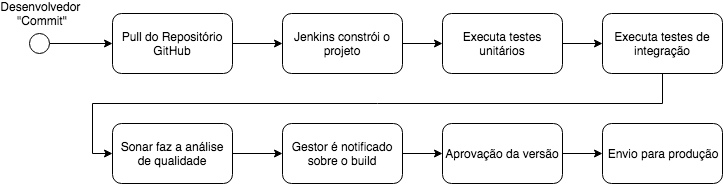
\includegraphics[width=1\linewidth]{imagens/pipelinebuild}
	\caption{Pipeline do Build}
	\label{fig:pipelinebuild}
\end{figure}


Durante todo o processo o SonarQube realiza o monitoramento e coleta dos resultados obtidos em todas as etapas do deploy, ao fim do processo é possível verificar nesse ambiente as estatísticas, tomando por base as métricas definidas. Isso dará uma visão mais próxima no que tange o desempenho e qualidade do deploy da aplicação.

\section{Pseudo-códigos dos Algoritmos Implementados}

Afim de organização os playbooks foram agrupados por categorias, sendo o playbook cd.yml o responsável pela chamada dos demais. Cada Playbook é constituído por diversas funções que identificam o tipo da dependência ou serviço, sua versão, se existe repositório específico ou se o Ansible fará a gestão deste, e a definição da tag que identifica a qual serviço essa função pertence.


O pseudo-código 1 faz menção a execução do playbook inicial do Ansible, nele será solicitado a execução de cada um dos demais playbooks que dizem respeito aos serviços necessário para o ambiente:

\begin{figure}[htb]
	\centering
	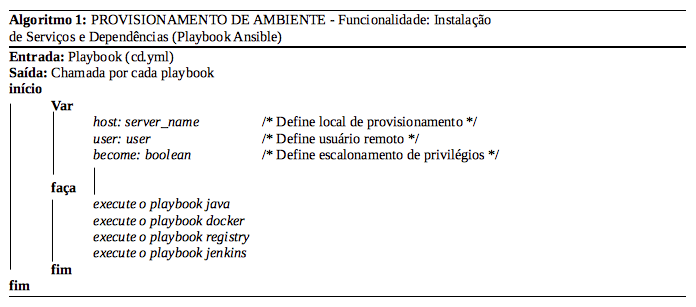
\includegraphics[width=1\linewidth]{imagens/algoritmo1}
\end{figure}

    \vspace*{2cm}

O Pseudo-código 2 trata da execução de cada playbook de serviço, onde verifica-se cada função que trata as dependências exigidas para que esse serviço possa funcionar:
\begin{figure}[htb]
	\centering
	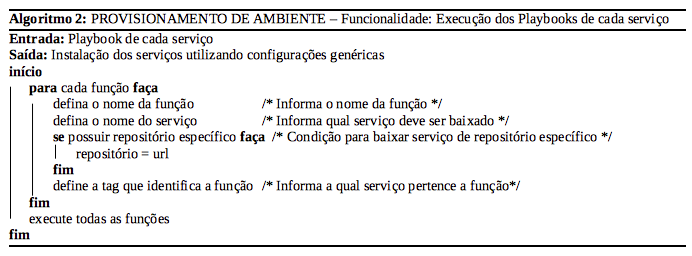
\includegraphics[width=1\linewidth]{imagens/algoritmo2}
\end{figure}

    \pagebreak[4]

O Pseudo-código 3 busca por Jobs em um diretório mapeado pelo contêiner Docker de cada serviço, nesse diretório serão armazenados os arquivos .json gerados com o preenchimento do formulário de solicitação de ambiente de desenvolvimento:	
\begin{figure}[htb]
	\centering
	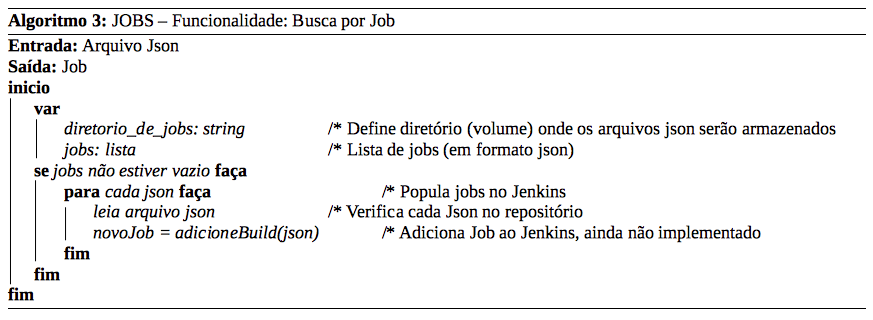
\includegraphics[width=1\linewidth]{imagens/algoritmo3}
\end{figure}

\vspace*{2cm}
    
O Pseudo-código 4 trata da execução dos Jobs no Jenkins, onde passa pela busca de jobs no diretório, baixa o código do repositório git informado no formulário, gera uma nova versão do código e se autorizado pelo gestor, executa o contêiner:	
\begin{figure}[htb]
	\centering
	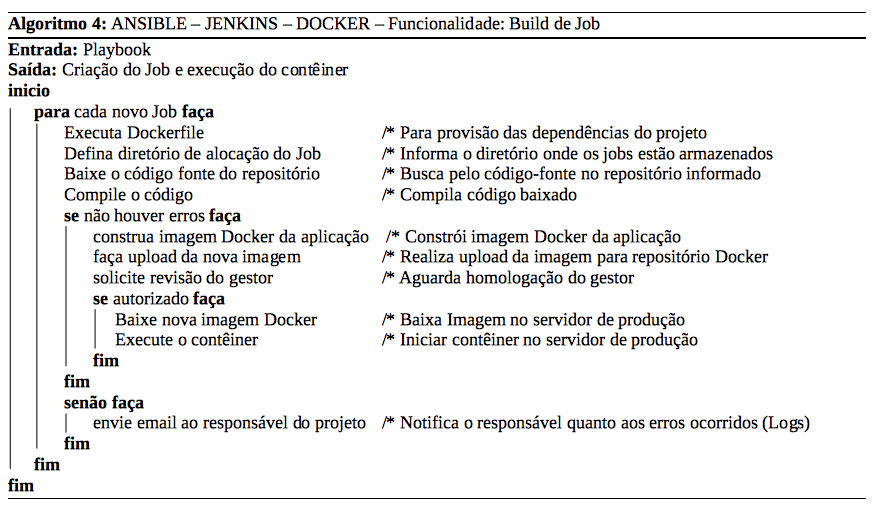
\includegraphics[width=1\linewidth]{imagens/algoritmo4}
\end{figure}



    \pagebreak[4]
\section{Métricas}

A definição de mecanismos que forneçam e possibilitem a análise estatística de todo o processo é fundamental dentro deste projeto. Nesse sentido, o uso de métricas é necessário para que se tenha uma visão próxima de cada processo de deploy. Serão adotadas nesse projeto as seguintes métricas expostas na tabela 3:


\begin{table}[h]
	\small
	\begin{tabular}{l|c}
		\hline
		\multicolumn{1}{c|}{MÉTRICA} & DESCRIÇÃO \\ \hline
		Tempo de Deploy & \begin{tabular}[c]{@{}c@{}}Critério utilizado para avaliar o tempo gasto para\\ uma atualização de aplicação entrar em produção\end{tabular} \\ \hline
		Taxa de erros & Ocorrência de erros retornados durante a execução\\dos Jobs. \\ \hline
		\begin{tabular}[c]{@{}l@{}}Desempenho frente a múltiplos\\ deploys\end{tabular} & \begin{tabular}[c]{@{}c@{}}Medição do desempenho obtido frente\\ à um estresse de deploys simultâneos\end{tabular} \\ \hline
		\begin{tabular}[c]{@{}l@{}}Recurso computacional \\consumido utilizando diferentes\\instâncias de Slaves.\end{tabular} & \begin{tabular}[c]{@{}c@{}}Quantidade de recursos de memória e processamento\\utilizados entre os slaves para concluir a tarefa iniciada.\end{tabular} \\ \hline
	\end{tabular}
\caption{Métricas Definidas}
\end{table}


Os resultados das métricas definidas são importantes pois com isso é possível ter noção muito próxima da "saúde" do código, pontos de fragilidade, potenciais melhorias, eventuais de melhorias nos recursos físicos e previsão de tempo de entrega de uma funcionalidade. Esses pontos dão suporte para tomadas de decisões por parte do gestor do projeto. Em se tratando do SonarQube a própria ferramenta já traz uma série de métricas pré-definidas e genéricas que podem ser aplicadas aos mais diversos tipos de jobs, e nesse ponto é importante ressaltar que é possível a criação de scripts específicos de testes de acordo com o tipo de tarefa que está sendo executada no build, no entanto o foco aqui não foi a implementação dos testes, mas sim a provisão do ambiente de automatização.

\chapter{Resultados}\label{cap:resultados}

Após análise das ferramentas estudadas e posteriormente eleitas as que melhores se adequaram ao presente estudo, partiu-se para a elaboração e concepção do modelo proposto para entrega de aplicação externa com base em uma visão DevOps.

A figura 5 representa a proposta de modelo de arquitetura para aplicação externa pretendida nesse estudo. O processo que dará início à sequencia de testes e deploy, começará com a requisição do usuário (desenvolvedor) para adquirir um repositório com intuito de armazenar uma determinada aplicação web. Isso quer dizer, que o programador terá acesso a um formulário de requisição (via sistema web) para pretensão de repositório, será retornado ao mesmo o link desse repositório a fim de que o mesmo possa hospedar o seu código. Os códigos e alterações serão enviados ao GitHub. Depois de enviar o código, o Jenkins receberá continuamente os códigos e executará os testes. Sendo os testes realizados com sucesso e tendo retorno positivo, sem erros, o Jenkins realizará o deploy no servidor através do Docker.





















\chapter{Conclusão}\label{cap:conclusao}

Este trabalho concentrou-se na apresentação dos conceitos da visão DevOps e analogia com o modelo tradicional de entrega de um software, onde ao decorrer do estudo analisou-se diversas ferramentas disponíveis no mercado e elegeram-se as que mais se adequavam à necessidade da implementação de um modelo de entrega para aplicação externa com o conceito de deploy automatizado.

O deploy automatizado fornece ao desenvolvedor e profissional de TI um ambiente simplificado para entrega de uma aplicação externa, tornando o gestor de tecnologia um provedor de serviço.

O presente modelo tem como foco contribuir para o aprimoramento no processo de entrega de software. Nesse sentido o cenário atual ainda lida com o processo de deploy baseado no modelo tradicional "cascata". Com o estudo realizado nesse projeto é possível otimizar o planejamento do processo da entrega da aplicação para produção utilizando recursos automatizados e gratuitos (open source) e uma visão DevOps. É possível economizar não só tempo como recursos humanos e financeiros que são fundamentais para a conclusão do processo.

Para continuidade deste projeto, objetiva-se a implementação de um cenário funcional utilizando máquinas virtuais, como expõe-se a seguir:

\begin{enumerate}
	\item Implementar o cenário apresentado neste projeto;
	\item Validar o modelo considerando diversas situações;
	\item Implementar o modelo visando ambientes críticos e cenários de risco.
	\item Implantar a solução afim de gerar um estudo de caso, visando verificar a aceitação da mesma.
\end{enumerate}


% ----------------------------------------------------------
% ELEMENTOS PÓS-TEXTUAIS
% ----------------------------------------------------------
\postextual
% ----------------------------------------------------------

% ----------------------------------------------------------
% Referências bibliográficas
% ----------------------------------------------------------
\bibliography{bibliografia}

%---------------------------------------------------------------------
\phantompart
\printindex
%---------------------------------------------------------------------

\end{document}
\grid

